\newlength{\bibsep}
\documentclass[nonatbib,5p,a4paper]{elsarticle}  % 5p for two columns, 1p for 1 column (this is specific for the elsearticle)
\usepackage[english]{babel}        % Language
\usepackage[DatePublished]{Code/NTNU-lab}        % remove [DatePublished] to remove dates
\usepackage{csquotes}                            % Must be loaded when babel is loaded to avoid error.
\input{Code/preamble}                            % Write all preamble code in this file to keep it organised and tidy.

\addbibresource{Bibliography/Sources.bib}        % Selects the Bibliography file.


\begin{document}
\selectlanguage{english}                         % Sets the language of the document.

%%%%%%%%%%%%%%%%%%%%%%%%%%%%%%%%%%%%%%%%

\begin{frontmatter}
%
% Title:
%------------------------------------
\title{%
SUTD Computer Vision (50.035) Final Report\\
\small Group 16  % A good idea is to have the subject code and name as subtitle
}
%
% Authors:
%------------------------------------
% List an author with name ' Firstname Middlename Lastname ' like this:
% F. M. Lastname
\author{Lee Le Xuan} 
\author{Keith Low}
\author{Issac Koh} 
\author{Aqif Yeo}
%
% Date:
%------------------------------------
%
\newdate{dateName}{13}{12}{2024} % edit the date here, ' dateName ' has to match on these two lines.
\renewcommand*{\today}{\MonthYearDateFormat\displaydate{dateName}} 
% Options for displaying date: \MonthYearDateFormat,  \DayMonthYearDateFormat or \YearDateFormat
%
% Abstract:
%------------------------------------
\NameOfAbstract{Abstract} % Change abstract title here. If you write in Norwegian, write 'Sammendrag' (nb) or 'Samandrag' (nn)
\begin{abstract}
% Delete the text and write your abstract here:
%------------------------------------

Understanding block diagrams is an often-overlooked challenge that requires complex functions such as deep-learning based computer vision and object detection methods. While these methods are effective for symbol detection, their reliance on bounding box representations poses challenges in recognizing line segments that are either very short or nearly parallel to the axes. In this report, we propose an improvement to the model developed by Bhushan and Lee by presenting a change in the Inception-ResNet-v2 backbone used in their paper. We compared the performances of using a Swin transformer and also introduced a new dataset for a wider variety of values.

\end{abstract}
%
\end{frontmatter}
%
%
% Table of contents:
%------------------------------------
% If the report is very long for some reason (over 4 or 5 pages), use a table of contents.
% Uncomment everything below the line ---- to get table of contents (ctrl + /) (the / on numberpad):
%-------------
%
% \ 
% \vspace{1cm}

% \begin{minipage}{\textwidth}
%     \tableofcontents
% \end{minipage}
% \clearpage
%\input{Text/0.2-Nomenclatures}                 % List of symbols, can be useful
\section{Introduction}
% Delete the text and write your Introduction here:
%------------------------------------



Block diagrams are a key medium to display complicated relationships or processes in an easy-to-read manner. These block diagrams have become more and more prevalent, often being included in user manuals, scientific papers and business process documentation. With a wider adoption of block diagrams in the current literature to display these complex situations, further flowchart recognition development is required for document analysis and recognition \cite{Griffiths}.

Block diagrams comprise of many complex shapes, lines or arrows that add to the complexity of understanding them using Document Artificial Intelligence (Document AI). They range from simple systems with few processes to highly interconnected subsystems, joined by numerous components. This poses a challenge for Document AI, which has many applications for document classification \cite{kang_2014_convolutional}, information extraction \cite{hwang2019postocr} and visual question answering (source). As a result, those with visual impairments may struggle to understand block diagrams, due to the difficult nature of recognizing and refining the structural semantics of block diagrams \cite{mathew_2020_docvqa}. 

In this paper, we propose a Swin transformer backbone to improve performance, with the goal of improving the work of  Shreyanshu and Lee \cite{bhushan-lee-2022-block}. The core idea of the improvement is to replace the Faster RCNN backbone proposed in their architecture, more specifically within the shape prediction of block diagrams. A block diagram generator was implemented along side the possible improvements, to add further complexity and variety for the model training. 




%\input{Text/0.1-Big_Figures}                    % Change this to another line to move big figures.
\section{Related Work}
% Delete the text and write your Theory/ Background Information here:
%------------------------------------

\subsection{Block Diagram Recognition}
Most prior studies of machine-generated block diagram recognition took place after the CLEF-IP in 2011, which was held by the Information Retrieval Facility (IFR) and released a public machine-generated flowchart dataset \cite{9795274}. Adams \cite{adams_2005_electronic} extracted the entire block diagram by analysing the connected components in images, before identifying specific structures using manually chosen features. This however would result in reduced accuracy when detecting incomplete (dotted lines) or broken edges. Mörzinger et al. \cite{mrzinger_2012_visual} first separated the diagram and text before studying the visual features of a structure, going to the pixel level.

For handwritten block diagrams, Julca-Aguilar and Hirata\cite{DBLP:journals/corr/abs-1712-04833} employed the Faster R-CNN for symbol detection. Results show that Faster R-CNN was effective on both publicly available flowchart and mathematical expression (CROHME-2016) datasets. Schäfer \cite{bernhardschfer_2021_arrow} built the first deep learning system for joint structure and symbol recognition in handwritten diagrams using Arrow R-CNN. 

On a similar vein, Farahani and colleagues \cite{alivasheghanifarahani_2023_automatic} reviewed recent automatic chart image understanding techniques more focused on charts (bar chart, pie chart, scatter plot). Shreyanshu and Lee \cite{bhushan-lee-2022-block} proposed a new framework for the summarization of block diagram images, called “Blosum”. The “Blosum” architecture would decompose the images into possible sets of triplets, capturing the relationships between components. 


\subsection{Transformer Architecture}
Transformer architectures have revolutionized computer vision tasks in recent years, with models like the Vision Transformer (ViT) and its derivatives achieving state-of-the-art performance across various domains. Unlike traditional convolutional neural networks (CNNs), which process spatially local information using kernels, transformers utilize self-attention mechanisms to capture global context within an image. This makes them particularly suited for recognizing structural relationships in block diagrams, where global context plays a vital role in understanding component interactions and spatial dependencies.

The Swin Transformer \cite{liu_2021_swin}, a hierarchical vision transformer, was introduced as a means to overcome the computational challenges associated with traditional transformer models. By adopting a shifted window mechanism, Swin Transformer processes images in smaller, non-overlapping windows while allowing information flow between adjacent windows. This approach ensures a fine balance between computational efficiency and the ability to model long-range dependencies. Such a capability is critical for block diagram recognition, where short and nearly parallel line segments often require an understanding of their global positioning within the diagram.

The rationale behind exploring the Swin Transformer for block diagram recognition lies in its ability to handle hierarchical representations effectively. Additionally, its adaptability to irregular shapes and non-uniform layouts aligns well with the inherent variability in block diagram structures.

 

 

 




\section{Proposed Approach}
% Delete the text and write your Method(s) here:
%------------------------------------
\subsection{Motivation}
Of all the papers that we examined, we were interested in the work done by Bhushan and Lee \cite{bhushan-lee-2022-block} on block diagram summarization capabilities. Although Blosum performed respectably well for the online generated block diagrams, it struggles mainly with hand-written texts. This was due to the version of EasyOCR not supporting handwritten texts and the focus of Blosum being on computerized block diagrams. Hence, our project would focus on improving the Blosum architecture to better detect handwritten text, to generate a better performance on the $FC\_A$ dataset. \par

Based on this, our project centers around modifying the existing architecture presented by Bhushan and Lee \cite{bhushan-lee-2022-block} to better detect handwritten block diagrams. Blosum is comprised of mainly four parts, as shown in the \Cref{fig:Blosum architure}. It consists of shape prediction, text prediction, arrow prediction and triplet generation. We propose that by experimenting with the backbone of the Blosum architecture, we may be able to derive better results with regards to the shape prediction, leading to a better performance on the $FC\_A$ dataset. 

\begin{figure}
    \centering
    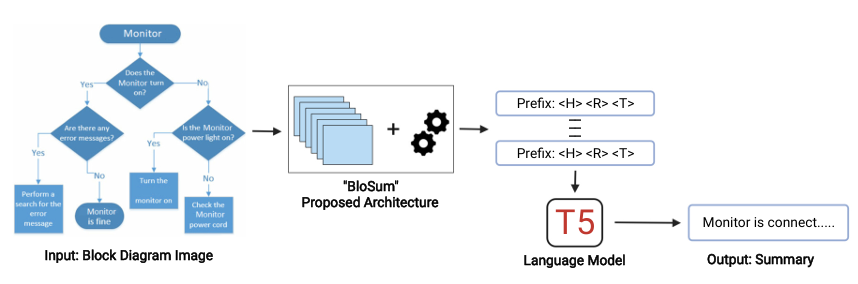
\includegraphics[width=0.48\textwidth]{Images/Blosum architecture.png}
    \caption{Blosum architecture proposed by Bhushan and Lee \cite{bhushan-lee-2022-block}.}
    \label{fig:Blosum architure}
\end{figure}


\subsection{Our Model}
Our architecture model explored in this project followed the architecture used Bhushan and Lee \cite{bhushan-lee-2022-block}. Focusing on the shape prediction portion, we substituted the Inception-ResNet-v2 backbone for a Swin transformer instead. 

The choice of the Swin transformer was due to its ability to deal with small visual entities and pixel level patterns. The Swin transformer can address these challenges by proposing hierarchical processing of image tokens using shifted window patches with linear complexity to image size \cite{singh_2024_swin}.  This hierarchical architecture has the flexibility to model at various scales and has linear computational complexity with respect to image size \cite{liu_2021_swin}, allowing greater performance when detecting arrowheads in block diagrams.


\subsection{Shape Prediction and Triplet Generation}
The shape prediction feature was treated as an object detection task. Similar to Bhushan and Lee \cite{bhushan-lee-2022-block}, for each shape $s \in S$, it predicts a bounding box $bs \in R4$ and a class name $cs \in C$. We defined seven plus one (background) different classes, which include Connection, Data, Decision, Terminator, and Process. 

The Inception-ResNet-v2 backbone here worked by having multi-level feature extraction that can capture information at various scales and complexities. Dimensionality reduction and pooling was also carried out to reduce the complexity and reduce over fitting respectively. To ensure fair testing, we also kept the similar intersection over union (IoU) threshold value of 0.8 over all shape classes. To prevent duplicates, a non-maximum suppression (NMS) was applied. 


Additionally, based on the information collected from the previous steps, we created a similar pipeline used to form a triplet generator. The generator would capture the relationship between the shapes detected by finding the closest anchor point placed on other shapes.


\section{Dataset}
% Delete the text and write your Results here:
%------------------------------------
\subsection{Dataset Used}
To ensure fairness in the improvement of our model, we opted to use the same computerized block diagram that was presented by the authors. This new dataset comprised of 502 diagrams and contained more than 13,000 annotated elements (shapes, edges, and text phrases) and was retrieved on GitHub. There are total 7 classes, each for a block element: Connection for circle, Data for parallelogram, Decision for diamond, Terminator for eclipse, Arrow, Text and Process for all other shapes not mentioned above. 

\subsection{Data Augmentation}
As highlighted previously, a key limiting factor that mitigated the performance of the original Inception-ResNet-v2 model was the difficulty of obtaining useful annotated data sets for object detection models. Despite scraping 502 images online, the manual task of annotating them with detailed labels (shapes, arrows, texts), bounding-boxes, and creating human-written summaries is labour-intensive and time-consuming. 

Additionally, the 502 images had limited variability as shown in Figure~\ref{fig: Class Instances of the CBD Dataset}. The dataset would not capture the full diversity of block diagrams, including different shapes, shape representations, text styles, and arrow connections. In this work, we propose to a data generation plan with an existing knowledge base and Mermaid graphing tool. With an additional new dataset, it would be able to help improve the generalization capabilities of our model compared to other datasets. 

\begin{figure}
    \centering
    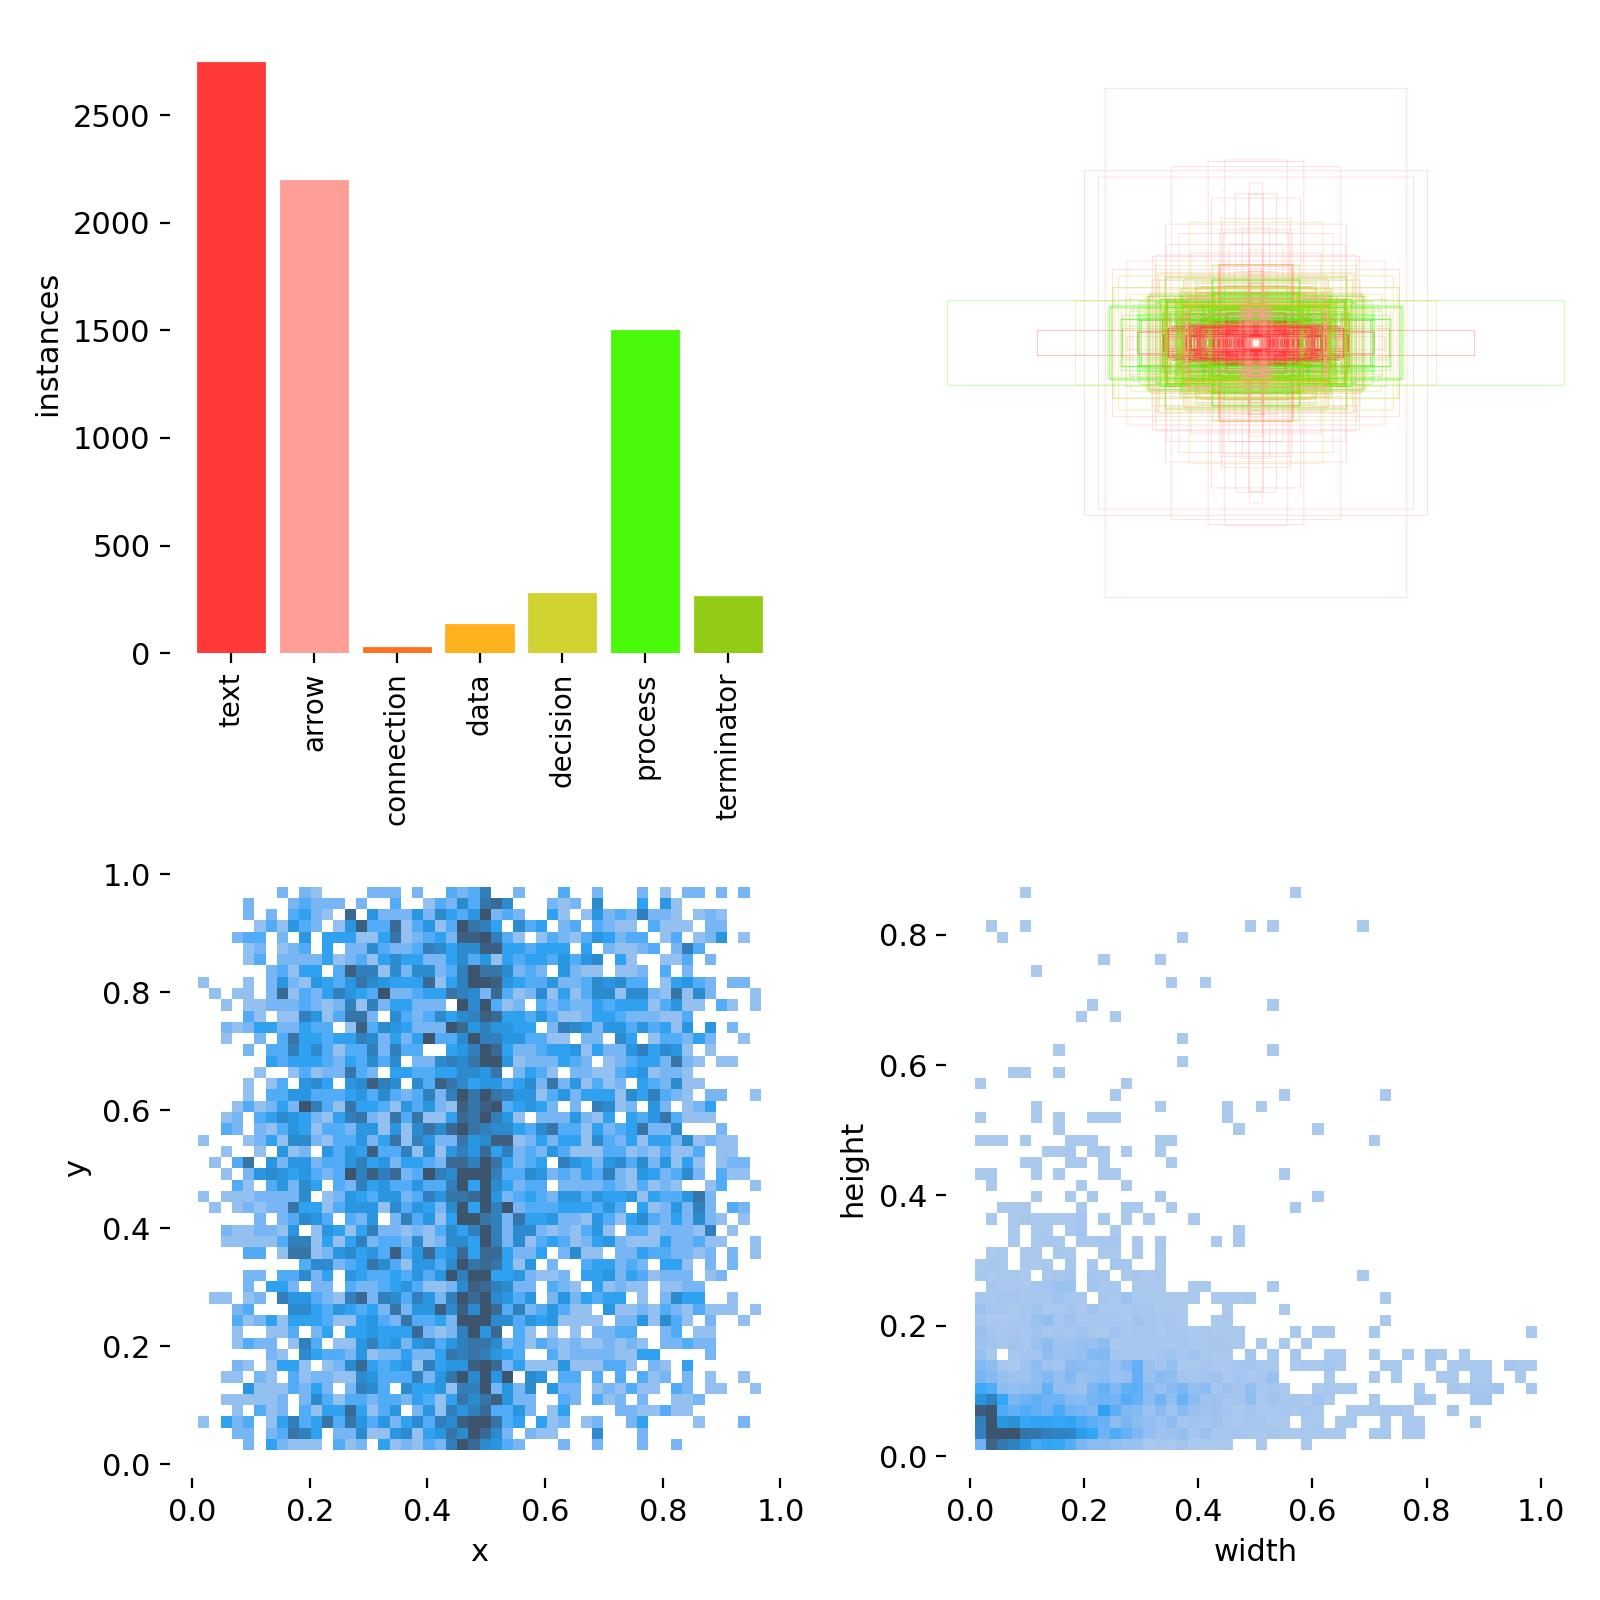
\includegraphics[width=0.48\textwidth]{Images/Class Representation.jpg}
    \caption{Class Instances of the CBD Dataset}
    \label{fig: Class Instances of the CBD Dataset}
\end{figure}


This ideally allows models to learn how to reverse engineer the entity-relation-entity triplets from the generated diagrams. For each entity-relation-entity triplet $x=[e_{1}, r, e_{2}]$, construct a directed graph $G = (V,E)$ such that there exists vertices $e_1,e_2 \in V$, a directed edge $(e_1,e_2) \in E$ with label $r$ for all $x \in X$, where $X$ represents set of all triplets in the knowledge graph. An pseudo-code version of this algorithm is shown in Figure~\ref{fig: Pseudo-code for the graph generation algorithm}. Finally, visualize this graph using certain visualization tools such as Mermaid, and easily obtain the labels and bounding-boxes for the diagram because of it's computerized nature.

\begin{figure}
    \centering
    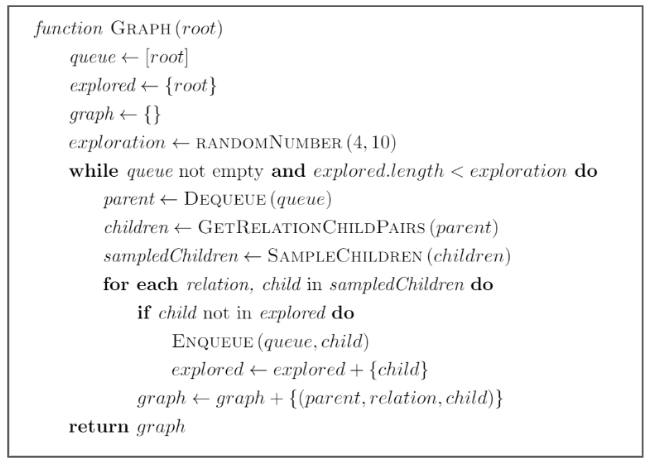
\includegraphics[width=0.48\textwidth]{Images/Graph generation algo.png}
    \caption{Pseudo-code for the graph generation algorithm}
    \label{fig: Pseudo-code for the graph generation algorithm}
\end{figure}






\begin{table*}
    \caption{Mean Average Precision per class score matrix on $FC\_A$}
    \label{tab:Map per class score}
    \centering
        \begin{tabular}{lccl}
        \hline
         & \multicolumn{1}{l}{Faster RCNN - Swin T} & \multicolumn{1}{l}{Faster RCNN - Inception-ResNet-v2} \\ \hline
        Text       & 0.44 & 0.25   \\
        Arrow      & 0.41 & 0.36   \\
        Connection & 0.11 & 0.00   \\
        Data       & 0.75 & 0.46   \\
        Decison    & 0.70 & 0.54   \\
        Process    & 0.63 & 0.61   \\
        Terminator & 0.85 & 0.07   \\ \hline
        \end{tabular}
\end{table*}

\begin{table*}
    \caption{Mean Average Recall per class score matrix on $FC\_A$}
    \label{tab:Mar per class score}
    \centering
        \begin{tabular}{lccl}
        \hline
         & \multicolumn{1}{l}{Faster RCNN - Swin T} & \multicolumn{1}{l}{Faster RCNN - Inception-ResNet-v2} \\ \hline
        Text       & 0.80 & 0.69   \\
        Arrow      & 0.81 & 0.74   \\
        Connection & 0.31 & 0.05   \\
        Data       & 0.85 & 0.67   \\
        Decison    & 0.84 & 0.72   \\
        Process    & 0.75 & 0.79   \\
        Terminator & 0.88 & 0.54   \\ \hline
        \end{tabular}
\end{table*}

\begin{table*}
    \caption{Confusion Matrix on $FC\_A$}
    \centering
    \label{tab:Confusion matrix}
        \begin{tabular}{lccl}
        \hline
         & \multicolumn{1}{l}{Faster RCNN - Swin T} & \multicolumn{1}{l}{Faster RCNN - Inception-ResNet-v2}  \\ \hline
        Precision (MAP) & 0.57 & 0.34   \\
        Recall (MAR)    & 0.77 & 0.62   \\
        F1 Score        & 0.66 & 0.44   \\ \hline
        \end{tabular}   
\end{table*}


\section{Implementation}
% Delete the text and write your Discussion here:
%------------------------------------
\subsection{Testing}
We trained on the test set of the computerized block diagrams, which had 300 images, and evaluated on FC-A, which is the handwritten dataset. This is to test out the generalizability of our models, and is also inline with testing done by the paper Blosum. 

\subsection{Evaluation Metrics}
For our evaluation, we calculated the F1-Score, Mean Average Precision (MAP) and Mean Average Recall (MAR). We set IOU=0.7, similar to the paper. 

These are the results we obtained are summarised in \cref{tab:Map per class score}, \cref{tab:Mar per class score} and \cref{tab:Confusion matrix}.




\subsection{Results}
The overall MAP of the model with Swin-Transformer backbone was higher than that of with the Inception-ResNet-v2 backbone, even though the Inception-ResNet-v2 managed to achieve a slightly higher MAP on the test set of the computerized block diagrams. This shows that the Swin-Transformer is able to generalize better. In addition, the overall training duration of the Swin-Transformer was twice as fast as that of the Inception-ResNet-v2. 

For both Inception and Swin-T models, the precision and recall for "Connection" are the lowest. This could be due to having less data for the "Connection" shapes, and we might not have ran enough epochs on both models to capture enough information. 

The MAP for the models are generally quite low as we only ran 50 epochs on both. This was due to time and resource constraints. 

Overall, the model with Swin-T as the backbone performed better.

For the data augmentation, we ran it 50 sets of it with 20 epochs on the Swin Transformer. Results was better by 0.02 MAP, and we can extrapolate this to 50 epochs to predict that the results would be better. 


\section{Limitations and Challenges}
% Delete the text and write your Conclusion here:
%------------------------------------


The detection of small or nearly parallel line segments, especially in crowded or dense block diagrams, remains a challenge. Despite the Faster RCNN's ability to capture fine-grained details, certain small features, such as tiny arrows or short lines, are still difficult to detect accurately. This issue is exacerbated in diagrams where these features are highly variable or not aligned to standard orientations.

Although the augmented dataset increased the variety of diagrams, there are still many non-standard diagram formats and visual representations that our model struggles to recognize effectively. Diagrams with unconventional shapes, inconsistent use of arrows, or text positioned outside the typical areas may lead to misclassification or detection failures.

\section{Sustainable Development Goals}

Our work presented in this project pushes Sustainable Development Goals number four and sixteen, Quality Education and Peace, Justice and Strong Institutions. With an easier way to summarize block diagrams through visual document understanding, this allows for automated content digitisations for greater accessibility to all. 

We believe that this would allow for better educational experiences for visually impaired learners through text descriptions or audio narration. Additionally, improving on process documentation can lead to the advancement of stronger institutes. Having an easier way to understand flowcharts can lead to easier management and efficient decision making. 
\section{Work Distribution}

\textbf{Le Xuan} - Implementation of the Inception-ResNet-v2 backbone for benchmark testing, implementation of the Swin transformer model, performed evaluation metrics for both backbones.\par

\textbf{Keith Low} - Data augmentation for the generation of a new dataset, implementation of the YOLOv5 backbone for benchmark testing, performed evaluation metrics for YOLOv5.\par

\textbf{Isaac Koh} - Research into Triplet generation, implementation of triplet with the Inception-ResNet-v2 backbone \par

\textbf{Aqif Yeo} - Report formatting and structure, research on implementation of Inception-ResNet-v2 backbone for benchmark testing. \par
\section{Conclusion}

This report aimed to improve the performance of an existing model by Bhushan and Lee to detect shapes in block diagrams. Our proposed model replaced the Inception-ResNet-v2 backbone model with a Swin transformer and a YOLOv5 model in the hopes of scoring a better F-measure, Precision and Recall score.  After testing with our own generated dataset, only the YOLOv5 model (98.4) yielded better results (96.24). This could be attributed to the one step interence in YOLOv5 compared to the two-step in Faster R-CNN. Although performing better, recognizing block diagrams and understanding the corresponding structural semantics with an end to-end model is still a hurdle.
%\clearpage                                     % Sometimes you want the rest on separate pages.
%\input{Text/Acknowledgements}                   % Comment out to exclude the Acknowledgements section

%%%%%%%%%%%%%%%%%%%%%%%%%%%%%%%%%%%%%%%%

% Bibliography
%--------------------
\printbibliography


\clearpage                                     % Sometimes it is useful to have appendix on separate page.
%\onecolumn                                     % If you want 1 column for appendix.
\appendix
\section{Triplet Generation}

We attempted to generate Head, Relation, Tail (\(<H> <R> <T>\)) triplets following the model proposed in BloSum \cite{bhushan-lee-2022-block}.

\begin{figure}[h]
    \centering
    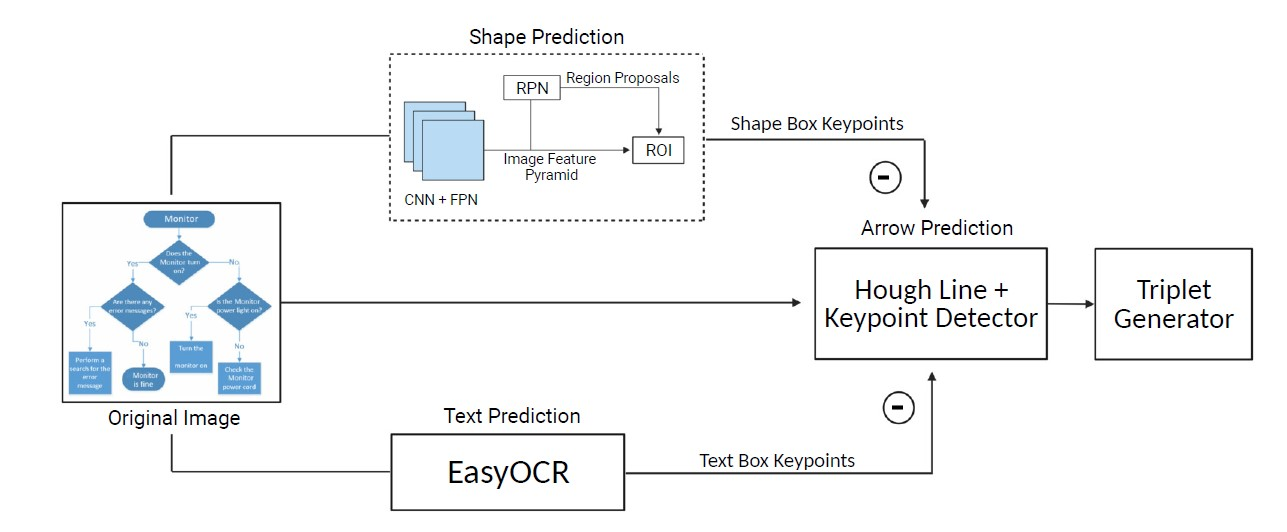
\includegraphics[width=0.48\textwidth]{Images/Triplet architecture.jpg} 
    \caption{Overall Architecture proposed in BloSum}
    \label{fig:appendix_triplet_architecture}
\end{figure}

\subsection{Text Prediction}

We used EasyOCR (Jaided, 2020) for detecting text \(T\) in an image. For each text \(t \in T\), it predicts a bounding box \(b_t \in \mathbb{R}^4\). We combined texts \(t\) where \(t\)'s bounding box falls within the bounding box of a shape \(s\).

\begin{figure}[h]
    \centering
    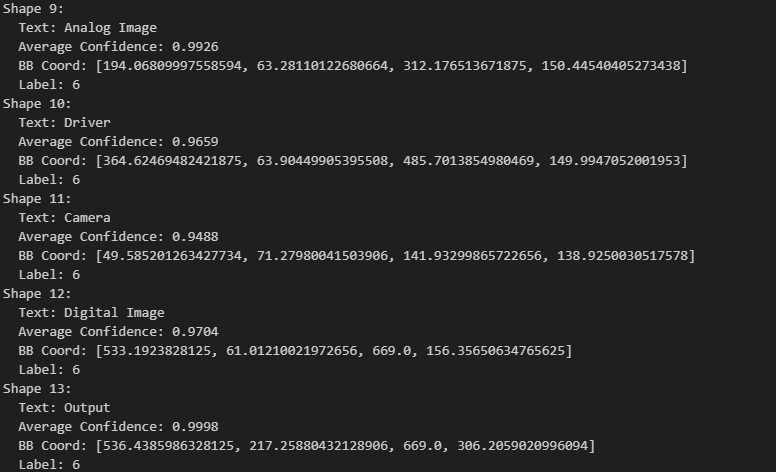
\includegraphics[width=0.48\textwidth]{Images/Sample output for easyOCR.jpg} 
    \caption{Sample Output for EasyOCR}
    \label{fig:appendix_isolated}
\end{figure}

\subsection{Arrow Prediction}

We subtracted non-arrow classes from the image before binarizing it to leave only the arrows behind. We then applied the Hough Line Transform to detect break and connecting arrows. We predicted the head and tail of an arrow by counting white pixels at the start and end points.

\begin{figure}[h]
    \centering
    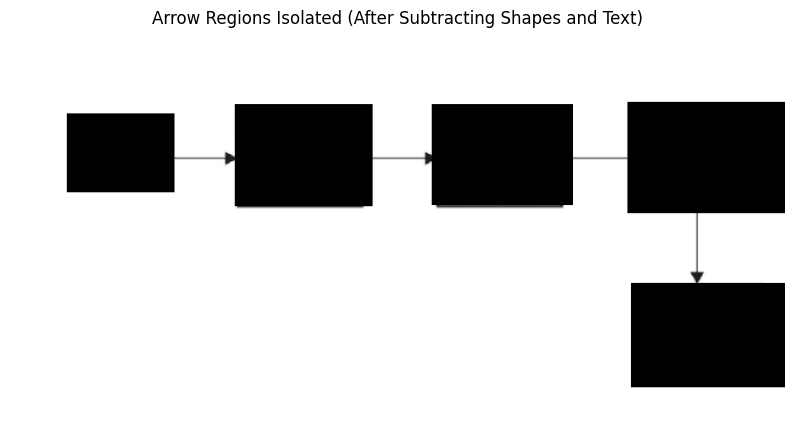
\includegraphics[width=0.48\textwidth]{Images/isolated.png} 
    \caption{Image after subtracting non-arrow classes}
    \label{fig:appendix_isolated}
\end{figure}

\begin{figure}[h]
    \centering
    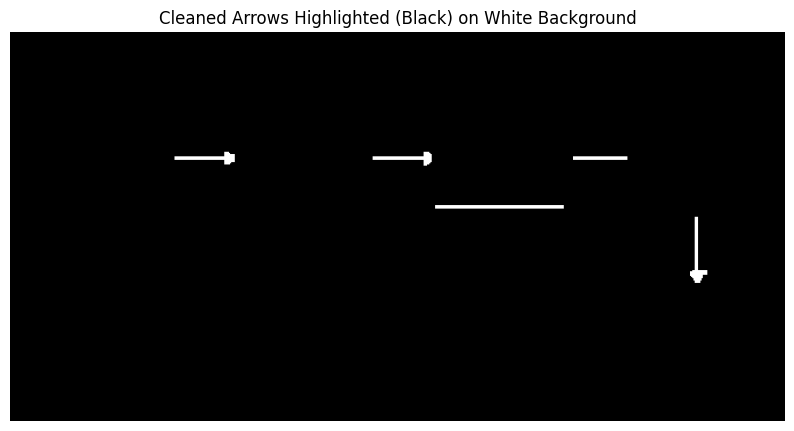
\includegraphics[width=0.48\textwidth]{Images/Binarized.png} 
    \caption{Image after Binarization}
    \label{fig:appendix_binarized}
\end{figure}

\subsection{Triplet Generator Logic}

We attempted to apply the same triplet generator logic used in BloSum \cite{bhushan-lee-2022-block}.

\begin{figure}[h]
    \centering
    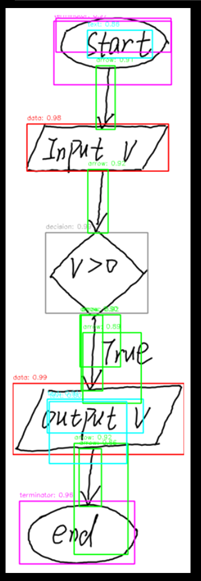
\includegraphics[width=0.48\textwidth]{Images/Fig Swin T CBD 50 epoch.png} 
    \caption{Fig Swin T CBD 50 epoch}
    \label{fig:appendix_binarized1}
\end{figure}

\begin{figure}[h]
    \centering
    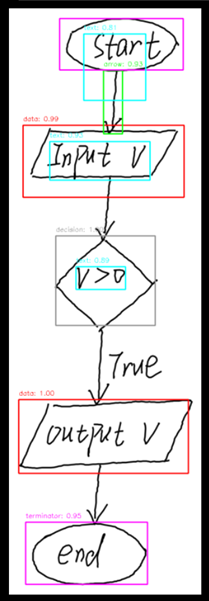
\includegraphics[width=0.48\textwidth]{Images/Swin t 100 epoch fca.png} 
    \caption{Swin t 100 epoch fca}
    \label{fig:appendix_binarized2}
\end{figure}

\begin{figure}[h]
    \centering
    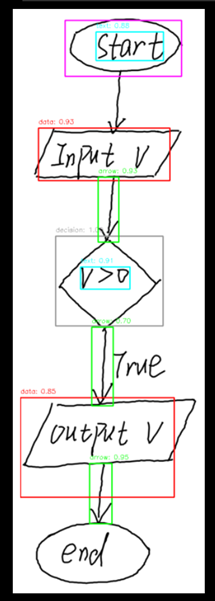
\includegraphics[width=0.48\textwidth]{Images/Inception Resnet 50 epochs.png} 
    \caption{Inception Resnet 50 epochs}
    \label{fig:appendix_binarized3}
\end{figure}



                           % Comment out to exclude appendix

\end{document}

% Copyright Remarks:
%--------------------

% Copyright holder: Vebjørn S. Førde, copyright: CC BY 4.0
% Note: The author of this template is also the copyright holder.

% Below is an explanation of the CC BY 4.0. Additional statements/ 
% clarifications made by the author/copyright holder are marked with *.

% YOU ARE FREE TO:
% Share — copy and redistribute the material in any medium or format
% Adapt — remix, transform, and build upon the material
% for any purpose, even commercially.

% UNDER THE FOLLOWING TERMS:
% Attribution* — You must give appropriate credit, provide a link to the license,
% and indicate if changes were made. You may do so in any reasonable manner, but 
% not in any way that suggests the licensor endorses you or your use.

% *Note: I do not need credit when the template is used to make a PDF document
% that is then distributed (like handing in a lab report). However, I would
% like for you to give credit if you choose to distribute the "software" 
% (the associated documentation files, .tex files and such). If you distribute
% both the PDF and the software, then you only need to give credit in the software
% distribution.
% I do not need credit for the plain text (text in output PDF). However, you should
% give me credit if you chose to use/ distribute any of the images in this document.

% No additional restrictions — You may not apply legal terms or technological 
% measures that legally restrict others from doing anything the license permits.

% NOTICES:
% No warranties are given.

% Disclaimer* (added by copyright holder):
% THE SOFTWARE IS PROVIDED "AS IS", WITHOUT WARRANTY OF ANY KIND, EXPRESS OR
% IMPLIED, INCLUDING BUT NOT LIMITED TO THE WARRANTIES OF MERCHANTABILITY,
% FITNESS FOR A PARTICULAR PURPOSE AND NONINFRINGEMENT. IN NO EVENT SHALL THE
% AUTHORS OR COPYRIGHT HOLDERS BE LIABLE FOR ANY CLAIM, DAMAGES OR OTHER
% LIABILITY, WHETHER IN AN ACTION OF CONTRACT, TORT OR OTHERWISE, ARISING FROM,
% OUT OF OR IN CONNECTION WITH THE SOFTWARE OR THE USE OR OTHER DEALINGS IN THE
% SOFTWARE.

% Read more about CC BY 4.0:
% https://creativecommons.org/licenses/by/4.0/